\documentclass[a4paper]{article}
\usepackage[pdftex]{hyperref}
\usepackage[latin1]{inputenc}
\usepackage[english]{babel}
\usepackage{a4wide}
\usepackage{amsmath}
\usepackage{amssymb}
\usepackage{algorithmic}
\usepackage{algorithm}
\usepackage{ifthen}
\usepackage{listings}
\usepackage{array}
\usepackage{tabu}
% move the asterisk at the right position
\lstset{basicstyle=\ttfamily,tabsize=4,literate={*}{${}^*{}$}1}
%\lstset{language=C,basicstyle=\ttfamily}
\usepackage{moreverb}
\usepackage{palatino}
\usepackage{multicol}
\usepackage{tabularx}
\usepackage{comment}
\usepackage{verbatim}
\usepackage{color}
\usepackage{graphicx}

%% pdflatex?
\newif\ifpdf
\ifx\pdfoutput\undefined
\pdffalse % we are not running PDFLaTeX
\else
\pdfoutput=1 % we are running PDFLaTeX
\pdftrue
\fi
\ifpdf
\fi
\ifpdf
\DeclareGraphicsExtensions{.pdf, .jpg}
\else
\DeclareGraphicsExtensions{.eps, .jpg}
\fi

\parindent=0cm
\parskip=0cm

\setlength{\columnseprule}{0.4pt}
\addtolength{\columnsep}{2pt}

\addtolength{\textheight}{5.5cm}
\addtolength{\topmargin}{-26mm}
\pagestyle{empty}

%%
%% Sheet setup
%% 
\newcommand{\coursename}{Computer Architecture and Programming Languages}
\newcommand{\courseno}{CO20-320241}
 
\newcommand{\sheettitle}{Homework}
\newcommand{\mytitle}{}
\newcommand{\mytoday}{{7 October}, 2019}

% Current Assignment number
\newcounter{assignmentno}
\setcounter{assignmentno}{4}

% Current Problem number, should always start at 1
\newcounter{problemno}
\setcounter{problemno}{1}

%%
%% problem and bonus environment
%%
\newcounter{probcalc}
\newcommand{\problem}[2]{
  \pagebreak[2]
  \setcounter{probcalc}{#2}
  ~\\
  {\large \textbf{Problem \textcolor{blue}{\arabic{assignmentno}}.\textcolor{blue}{\arabic{problemno}}} \hspace{0.2cm}\textit{#1}} \refstepcounter{problemno}\vspace{2pt}\\}

\newcommand{\bonus}[2]{
  \pagebreak[2]
  \setcounter{probcalc}{#2}
  ~\\
  {\large \textbf{Bonus Problem \textcolor{blue}{\arabic{assignmentno}}.\textcolor{blue}{\arabic{problemno}}} \hspace{0.2cm}\textit{#1}} \refstepcounter{problemno}\vspace{2pt}\\}

%% some counters  
\newcommand{\assignment}{\arabic{assignmentno}}

%% solution  
\newcommand{\solution}{\pagebreak[2]{\bf Solution:}\\}

%% Hyperref Setup
\hypersetup{pdftitle={Homework \assignment},
  pdfsubject={\coursename},
  pdfauthor={},
  pdfcreator={},
  pdfkeywords={Computer Architecture and Programming Languages},
  %  pdfpagemode={FullScreen},
  %colorlinks=true,
  %bookmarks=true,
  %hyperindex=true,
  bookmarksopen=false,
  bookmarksnumbered=true,
  breaklinks=true,
  %urlcolor=darkblue
  urlbordercolor={0 0 0.7}
}

\begin{document}
\coursename \hfill Course: \courseno\\
Jacobs University Bremen \hfill \mytoday\\
Fjolla Dedaj\hfill
\vspace*{0.3cm}\\
\begin{center}
{\Large \sheettitle{} \textcolor{blue}{\assignment}\\}
\end{center}

\problem{}{0}
\solution
\\
The boolean expression of the circuit is: X = (A XOR B) $\wedge$ (B XNOR C) $\wedge$ C\\
\\
\begin{tabu} to 1.1\textwidth { | X[c] | X[c] | X[c] | X[c] | X[c] | X[c] | }
 \hline
 A & B  & C & A XOR B & B XNOR C &  X  \\
 \hline
 $0$  & $0$  & $0$  & $0$ & $1$ & $0$\\
 \hline
 $0$  & $0$  & $1$ & $0$ & $0$ & $0$\\
 \hline
 $0$  & $1$  & $0$ & $1$ & $0$ & $0$\\
 \hline
 $0$  & $1$  & $1$ & $1$ & $1$ & $1$\\
 \hline
 $1$  & $0$  & $0$  & $1$ & $1$ & $0$\\
 \hline
 $1$  & $0$  & $1$ & $1$ & $0$ & $0$\\
 \hline
 $1$  & $1$  & $0$ & $0$ & $0$ & $0$\\
 \hline
 $1$  & $1$  & $1$ & $0$ & $1$ & $0$\\
\hline
\end{tabu}\\
\\
\\
As it is evident from the truth table, X = 1 if we have the following input condition: $\mathbf{\overline{A} \wedge B \wedge C}$
\\
\problem{}{0}
\solution
\\
Boolean Expression from the circuit: $\overline{AB + C}$  XOR  $(\overline{A} * (B + C)) $\\
\\
\textbf{a)} Truth Table:
\\
\\
\begin{tabu} to 1.1\textwidth { | X[c] | X[c] | X[c] | X[c] | X[c] | X[c] | }
 \hline
 A & B  & C & $\overline{AB + C}$ & $(\overline{A} * (B + C)) $ &  X  \\
 \hline
 $0$  & $0$  & $0$  & $1$ & $0$ & $1$\\
 \hline
 $0$  & $0$  & $1$ & $0$ & $1$ & $1$\\
 \hline
 $0$  & $1$  & $0$ & $1$ & $1$ & $0$\\
 \hline
 $0$  & $1$  & $1$ & $0$ & $1$ & $1$\\
 \hline
 $1$  & $0$  & $0$  & $1$ & $0$ & $1$\\
 \hline
 $1$  & $0$  & $1$ & $0$ & $0$ & $0$\\
 \hline
 $1$  & $1$  & $0$ & $0$ & $0$ & $0$\\
 \hline
 $1$  & $1$  & $1$ & $0$ & $0$ & $0$\\
\hline
\end{tabu}
\\
\\
\\
\textbf{b)} Sum of products: $\mathbf{\overline{ABC} + \overline{AB}C + \overline{A}BC + A\overline{BC}}$\\
\problem{}{0}
\solution
\\
\\
\textbf{a)} $+27_{10} = \mathbf{00011011}$\\
\\
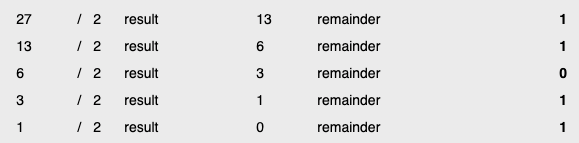
\includegraphics[scale=0.6]{27.png}
\\
\\
\pagebreak
\\
\textbf{b)} $+66_{10} = \mathbf{01000010}$\\
\\
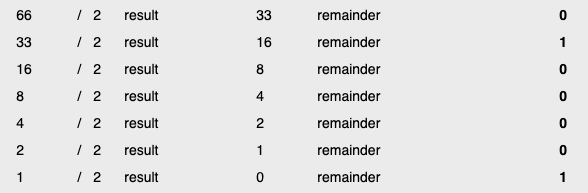
\includegraphics[scale=0.6]{66.png}
\\
\\
\textbf{c)} $-18_{10} = \mathbf{11101110}$\\
\\
Convert the positive version of the number to a binary representation: $18_{10} = 00010010_2$\\
\\
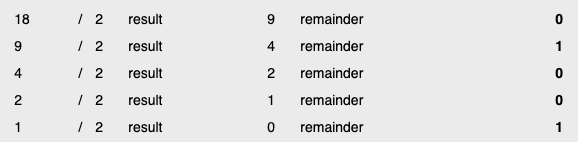
\includegraphics[scale=0.6]{18.png}
\\
\\
Flip the bits: $!(00010010) = 11101101$\\
\\
Add 1: $-18_{10} = 11101101 + 00000001 = \mathbf{11101110}$\\
\\
\\
\textbf{d)} $127_{10} = \mathbf{01111111}$\\
\\
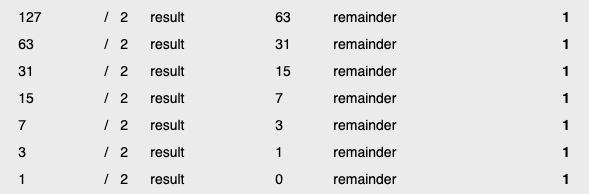
\includegraphics[scale=0.6]{127.png}
\\
\\
\textbf{e)} $-127_{10} = 10000001$\\
\\
Convert the positive version of the number to a binary representation: $127_{10} = 01111111_2$\\
\\
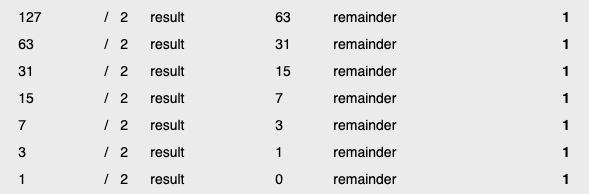
\includegraphics[scale=0.6]{127.png}
\\
\\
Flip the bits: $!(01111111) = 10000000$\\
\\
Add 1: $-127_{10} = 10000000 + 00000001 = \mathbf{10000001}$\\
\\
\pagebreak
\\
\\
\textbf{f)} $-128_{10} = 10000000$\\
\\
Convert the positive version of the number to a binary representation: $128_{10} = 10000000_2$\\
\\
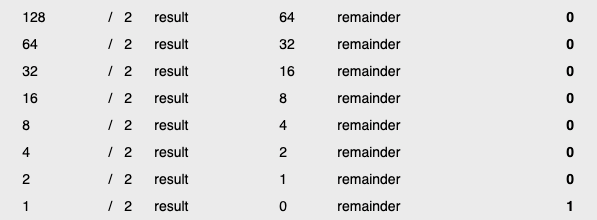
\includegraphics[scale=0.6]{128.png}
\\
\\
Flip the bits: $!(10000000) = 01111111$\\
\\
Add 1: $-128_{10} = 01111111 + 00000001 = \mathbf{10000000}$\\
\\
\\
\textbf{g)} $+131_{10} = \mathbf{10000011}$ As it is evident, the number is positive and after converting by using only 8 bits we get a binary number where the most significant bit is 1, meaning that it is negative. Thus, in this case we have an overflow.\\
\\
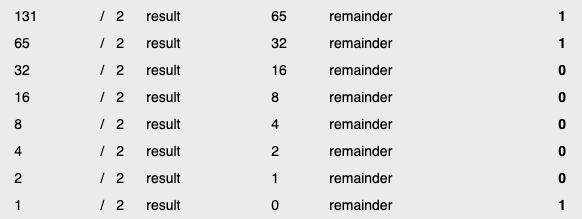
\includegraphics[scale=0.6]{131.png}
\\
\\
\textbf{h)} $-7_{10} = 11111001$\\
\\
Convert the positive version of the number to a binary representation: $7_{10} = 00000111_2$\\
\\
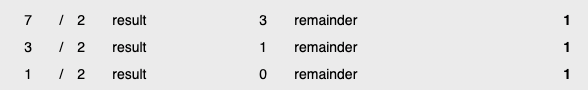
\includegraphics[scale=0.6]{7.png}
\\
Flip the bits: $!(00000111) = 11111000$\\
\\
Add 1: $-7_{10} = 11111000 + 00000001 = \mathbf{11111001}$\\
\\
\problem{}{0}
\solution
\\
\textbf{a)} $00011000 = 24_{10}$\\
\\
The number is positive, only the conversion to decimal is needed:\\
\\
$00011000 = (0 * 2^{7}) + (0 * 2^{6}) + (0 * 2^{5})+ (1 * 2^{4})+ (1 * 2^{3})+ (0 * 2^{2})+ (0 * 2^{1})+ (0 * 2^{0})=\mathbf{24_{10}}$\\
\\
\pagebreak
\\
\\
\textbf{b)} $11110101 = -11_{10}$\\
\\
Value is negative because it starts with 1.\\
\\
Flip the bits: $!(11110101) = 00001010$\\
\\
Add 1: $00001010 + 1 = 00001011$\\
\\
Convert to decimal and add the minus: $00001011 = (1 * 2^{3}) + (0 * 2^{2}) + (1 * 2^{1}) + (1 * 2^{0}) = \mathbf{-11_{10}}$\\
\\
\\
\textbf{c)} $01011011 = 91_{10}$\\
\\
The number is positive, only the conversion to decimal is needed:\\
\\
$01011011 = (0 * 2^{7}) + (1 * 2^{6}) + (0 * 2^{5}) + (1 * 2^{4}) + (1 * 2^{3}) + (0 * 2^{2}) + (1 * 2^{1}) + (1 * 2^{0}) = \mathbf{91_{10}}$\\
\\
\\
\textbf{d)} $10110110 = -74_{10}$\\
\\
Value is negative because it starts with 1.\\
\\
Flip the bits: $!(10110110) = 01001001$\\
\\
Add 1: $01001001 + 1 = 01001010$\\
\\
Convert to decimal and add the minus: $01001010 = (0 * 2^{7}) + (1 * 2^{6}) +(0 * 2^{5}) +(0 * 2^{4}) +(1 * 2^{3}) +(0 * 2^{2}) +(1 * 2^{1}) +(0 * 2^{0}) =\mathbf{-74_{10}}$\\
\\
\\
\textbf{e)} $11111111 = -1_{10}$\\
\\
Value is negative because it starts with 1.\\
\\
Flip the bits: $!(11111111) = 00000000$\\
\\
Add 1: $00000000 + 1 = 00000001$\\
\\
Convert to decimal and add the minus: $00000001 = (1 * 2^{0}) = \mathbf{-1_{10}}$\\
\\
\\
\textbf{f)} $01101111 = 111_{10}$\\
\\
The number is positive, only the conversion to decimal is needed:\\
\\
$01101111 = (0 * 2^{7}) + (1 * 2^{6}) + (1 * 2^{5}) + (0 * 2^{4}) + (1 * 2^{3}) + (1 * 2^{2}) + (1 * 2^{1}) + (1 * 2^{0}) = \mathbf{111_{10}}$\\
\\
\\
\textbf{g)} $10000001 = -127_{10}$\\
\\
Value is negative because it starts with 1.\\
\\
Flip the bits: $!(10000001) = 01111110$\\
\\
Add 1: $01111110 + 1 = 01111111$\\
\\
Convert to decimal and add the minus: $01111111 = (0 * 2^{7}) + (1 * 2^{6}) + (1 * 2^{5})+ (1 * 2^{4})+ (1 * 2^{3})+ (1 * 2^{2})+ (1 * 2^{1})+ (1 * 2^{0}) = \mathbf{-127_{10}}$\\
\\
\pagebreak
\\
\\
\textbf{h)} $10000000 = -128_{10}$\\
\\
Value is negative because it starts with 1.\\
\\
Flip the bits: $!(10000000) = 01111111$\\
\\
Add 1: $01111111 + 1 = 10000000$\\
\\
Convert to decimal and add the minus: $10000000 = (1 * 2^{7}) = \mathbf{-128_{10}}$\\
\problem{}{0}
\solution\\
For any addition greater than $9_{10}$, add binary equivalent of 6 to the Binary sum obtained and get its BCD equivalent (the comma operator distinguishes the digits):\\
\\
$27 + 36 = 0010,0111_{BCD} + 0011,0110_{BCD} = 0101,1101 + 0000,0110 = \mathbf{0110,0011_{BCD}} = 63_{10}$\\
\\
\\
$73 + 29 = 0111,0011_{BCD} + 0010,1001_{BCD} = 1001,1100 + 0000,0110 = 1010,0010 + 0110,0000 = \mathbf{0001,0000,0010_{BCD}} = 102_{10}$\\
\\
\\
\problem{}{0}
\solution\\
\textbf{a) What is the range of unsigned decimal numbers that can be represented by using 8 bits?}\\
\\
The range is $0$ to $255$ because the biggest number can be expressed as $11111111_2 = 255_{10}$ and the smallest one is $00000000_2 = 0_{10}$. In general, an m-bit unsigned number represents all numbers in the range $0$ to $2^{m} - 1$.\\
\\
\textbf{b) What is the range of signed decimal numbers that can be represented by using 8 bits (including the sign bit)?}\\
\\
The simplest case is to use 1 sign bit and 7 value bits. The range is $-127$ to $127$ because the biggest number can be expressed as $01111111_2 = 127_{10}$ and the smallest one is $11111111_2 = -127_{10}$ considering that the most significant bit is the sign bit.\\
\\
\textbf{c) What is the range of unsigned decimal numbers that can be represented by using 11 bits?}\\
\\
The range is $0$ to $2047$ because the biggest number can be expressed as $11111111111_2 = 2047_{10}$ and the smallest one is $00000000_2 = 0_{10}$. In general, an m-bit unsigned number represents all numbers in the range $0$ to $2^{m} - 1$.\\
\\
\textbf{d) What is the range of signed decimal numbers that can be represented by using 11 bits (including the sign bit)?}\\
\\
The simplest case is to use 1 sign bit and 10 value bits. The range is $-1023$ to $1023$ because the biggest number can be expressed as $01111111111_2 = 1023_{10}$ and the smallest one is $11111111111_2 = -1023_{10}$ considering that the most significant bit is the sign bit.\\
\\
\textbf{e) What is the range of signed decimal numbers that can be represented by using 16 bits (including the sign bit)?}\\
\\
The simplest case is to use 1 sign bit and 15 value bits. The range is $-32767$ to $32767$ because the biggest number can be expressed as $0111111111111111_2 = 32767_{10}$ and the smallest one is $1111111111111111_2 = -32767_{10}$ considering that the most significant bit is the sign bit.\\

\end{document}